\documentclass{tufte-handout}
\usepackage{graphicx}
\usepackage{amsmath}
\graphicspath{ {./images/} }
\renewcommand{\vec}[1]{\mathbf{#1}} %make \vec command turn vectors bold instead

\author{Andr\'es Ponce}
\title{Ensemble Methods}

\begin{document}
\maketitle
\begin{abstract}
	\textbf{Ensemble Methods} refer to when we use an aggregate of $L$ different
	models to find more accurate predictions for our data. There are several 
	ways of implementing a selection from several methods: adaboost, decision trees,
	bagging, random forests, etc...	
\end{abstract}

\section{Boosting}
The straightforward approach to using multiple models is to take the average value of each of the 
models that we use. Supposing we want to use $M$ models, and we want to predict the value given 
by a certain function, we could say 
\[y_{COM} = \frac{1}{M} \sum_{m = 1}^{M}y_{m}(x)\]

where $COM$ refers to the \textit{decision by committee} given by the equations. We take the average
value of the $M$ models to form our final result. When calculating the error, we also take the aggregate
error of all the models.

\textbf{Boosting} then refers to the building of a strong classifier for a problem by using several weaker
classifiers. When boosting, we again can have $M$ models whose scores are summed up. 

\begin{marginfigure}
	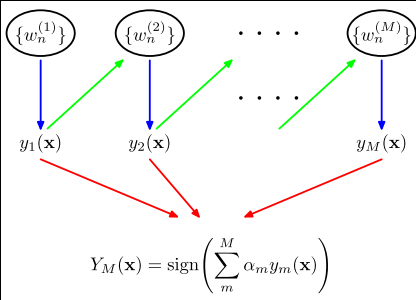
\includegraphics[scale=0.4]{adaptive}
	\caption{Each of the models contributes to how we pass the input set to the next model to be trained. 
	At the end, we also use each model's results to calculate the final prediction.}
\end{marginfigure}
The type of boosting called \textbf{Adaptive Boosting} will pass the input through the models
sequentially, and \textit{train} the models sequentially. Then, when training the next model, items that 
were misclassified will be given greater weight. This may result in an overall model which performs 
very well even if the models themselves perform as well as random ones.

The process for AdaBoost looks something like:
\begin{enumerate}
	\item Given inputs $(x_{1}, y{1}),...,(x_{m},y_{m})$ where $x_{i} \in X, y_{i} \in\{-1, +1\}$,
			initialize their distributions $D_{t}(i)= \frac{1}{m}, i = 1,...,m$
			\footnote{The distributions $D_{t}(i)$ mean the probability distribution of $x_{i}$'s at time $t$}
	\item Find the classifier $h_{t}$ which minimizes the error w.r.t. $D_{t}$.\footnote{We can basically take
			the min of 
				\[\epsilon_{j} = \sum_{i = 1}^{m}D_{t}(i)[y_{i} \neq h_{j}(x_{i})]\]}
	\item Calculate the weight classifier $\alpha_{t} = \frac{1}{2}ln\frac{1 - \epsilon_{t}}{\epsilon{t}}$
	\item Update our distribution \footnote{ $Z_{t}$ is basically a value to normalize the distribution.}
			\[ D_{t + 1}(i) = \frac{D_{t}\textrm{exp}[-\alpha_{t}y_{i}h_{t}(x_{i})]}{Z_{t}} \]
\end{enumerate}

Once we have the final classifier $H(x)$, comprised of the sum of the modesl with the adjusted weights and
distributions, we can calculate the \textbf{margin} of the classifier on a sample $(x, y)$. The margin is
given by \footnote{The margin tells us when we classified the input correctly, and our confidence with our 
classification.}
\[yH(x)\]

The AdaBoost algorithm will try to maximize the margins of our variables by minimizing the 
\textbf{exponential loss} of the predictions.
\[loss_{exp}[H(x)]= E_{x,y}[e^{-yH(x)}]\]

\section{Face Detection using AdaBoost}
To perform facial detection on an image, we can use \textbf{sliding windows} which apply some model to 
different portions of the image. However, this approach might be a bit challenging because of the 
large amount of areas that we would need to detect in a single image. Since the amount of pixels might be
very large, we would need to beware of the amount of false-positives that are possible. For this problem,
the \textbf{Viola-Jones} method is quite useful.
\subsection{Viola-Jones Face Detector}

The Viola-Jones method for detecting faces relies on finding \textbf{rectangle features} in images.
Since a face can have eyes, nose, etc... we can measure the difference in pixel areas between similar pattern
across faces. For example, if we have an idea of how different the eyes and nose should look like, we can use
a model similar to Figure \ref{fig:features} to measure that area. If the end result is something which we might
expect, then we can feel confident in saying there is a face or other feature inside.

\begin{marginfigure}
		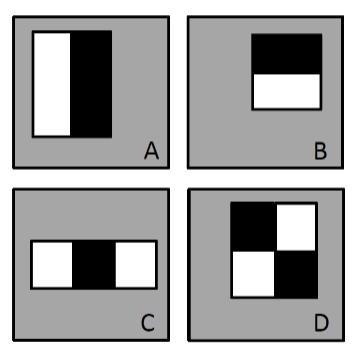
\includegraphics[scale=0.3]{rect_features}	
		\caption{In Viola-Jones, there are four types of features of rectangular features. Different
			models might be applicable to different parts of the face.We have to take
			the difference of the clear and the black areas. C might be used to measure eyes and nose area;
			B for eyes and mouth, etc...
			\label{fig:features}
			}
\end{marginfigure}

A ``feature" in Viola-Jones corresponds to a difference in pixel values. That's why having different models
with clear/black parts is useful: it can help us detect different parts in a face. Thus, for a feature value
$f(x)$ given an input image vector $x$ can be written as:

\[ \textrm{Feature Value} = \sum{}^{}(\textrm{Pixels in white area}) - \sum_{}^{}(\textrm{Pixels in black area}) \]

The next distinguishing feature of Viola-Jones facial recognition involves the \textbf{integral image}.This
aspect involves keeping a record of the sum of all preceding parts of an image. For an integral image $ii$,
the value $ii(x, y)$ is the sum of all values \textit{above and to the left of x, y}. 

\begin{marginfigure}
		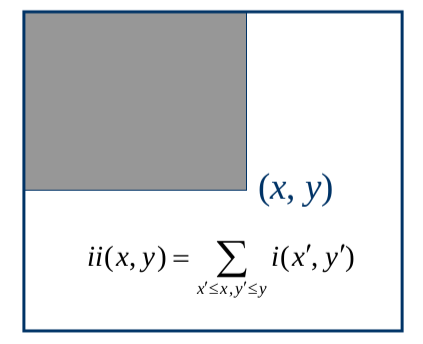
\includegraphics[scale=0.3]{integral}
		\caption{The value at $ii(x, y)$ is the sum of all the values that came before it.}
\end{marginfigure}

This way of storing cumulative image values makes finding the overall value in a rectangular area quite easy. 
In the end, we only need a constant number of additions to calculate the feature value of any rectangular 
area in our image.

\subsection{Boosting for face detection}
So far, we've only used Viola-Jones to detect faces through the integral image. Then how do we use boosting
with this approach? Similar to the definition covered before, we can use each one of the different classifiers
for the rectangle areas. We can constuct a weak learner such that \footnote{Remember a weak learner will just
work on a single recatangle area with the image.}

\[h(x) =  
	\begin{cases}
			1 & p_{t}f_{t} > p_{t}\theta_{t} \\
			0 & \textrm{otherwise}
	\end{cases}
\]
where $p_{t}$ is the polarity, $f_{t}(x)$ is the value of the rectangle feature, and $\theta_{t}$ is some
threshold. $\theta_{t}$ gives us our decision boundary. Thus we have over 160,000 weak learners.
This face detector has complexity $O(MNK)$ for its training cycle, where $M$ is the number of iterations,
$N$ is the training examples, and $K$ is thnumber of rectangle features.
The procedure for Viola-Jones boosting can be summarized as:
\begin{enumerate}	
	\item Evaluate the \textbf{feature rectangle} on each example.
	\item select best \textbf{threshold/parity} for each rectangle feature
	\item Select best \textbf{threshold/parity/rectangle-feature combination}
	\item Reweigh examples
\end{enumerate}
\section{Attentional Cascade}
With an \textbf{Attentional Cascade},the idea is to run a sub window of an image through increasingly strict
classifiers, and reject it as soon as one of the classifiers returns negative. With this approach, the rate
of \textbf{false positives} is the product of the false positive rates of each individual classifier, which may
be very little in the end.
\section{Decision Trees}
With \textbf{decision trees}, the idea is to split the space and traverse it in the same way we would a binary tree.
We use a divide-and-conquer approach.\footnote{Remember a dnd splits the problem into smaller instances, }
The idea is we have some function $f_{m}(x)$ at each tree node, and depending on its result we take one branch. 
We continue this until we reach a leaf node and can make a classification.

The way a decision is made with a tree might seem quite natural to humans, since analyzing one 
variable at a time might seem more intuitive to make a decision..
\subsection{Decision Tree Induction}
To build the tree, we could first start by splitting the data into two sections, and then recursively try to 
split the two subsets of data themselves. We stop adding nodes when some criterion is met for the error, or 
as a function of the input size and  model complexity. At each decison node, we can either look at
\textbf{univariate} attributes or \textbf{multivariate}.

Once we start splitting the dataset, we can measure its level of \textbf{purity} by seeing if for every class
$C_{k}$ there are any data points in its space that do not belong to it, that belong to another class $C_{p}$,
for example. We can measure the uncertainty and impurity by the following formula: \footnote{$p_{m}^{k}$ gives
the probability of class $C_{k}$}
\[ I_{m} = - \sum_{k = 1}^{K} p_{m}^{k} \log p_{m}^{k}\]

At every decision node, we have a decision to make based on a \textbf{threshold}. In practice, decision trees
might sometimes tend to overfit the training data. However, \textbf{bagging} and \textbf{random forests}
might help make decision trees more robust and easier to compute.

\section{Bagging}
With \textbf{bagging}, we take a sample set of size $D$, and we further split it into $m$ subsets by 
randomly sampling the original dataset \textbf{with replacement}. We then create separate classifiers
with the different datasets and combine them in some way during the final stage to make our final 
classifier.

\section{Random Forests}
When using random forests, we have to introduce two new sources of randomness: \textbf{bagging} and
\textbf{random vectors}. The latter refers to calculating a randomly selected subset of points 
and calculating the best split for each of those random vectors. How do we create a decision node?
There are a few methods:
\begin{itemize}
		\item Choose $m$ attributes randomly and calculate the one with the biggest possible \textbf{gain}
		\item If $M$ remains small, then we can choose $L$ attributes and calculate a linear combination of 
				those attributes that fall within $[1, -1]$.
		\item Compute the information gain of all the $M$ attributes and select the top $m$ by their information
				gain. Then randomly select one from within those $m$.
\end{itemize}
Where there are $M$ data dimensions, and $m < M$, $L\leq M$.

For the first method, we would have to for each number in $B$\footnote{The number of datasets we want to split 
$D$ into.} grow a decision tree based on the	best attribute at each node. Then we split the dataset into two
new child nodes.
\end{document}
